We use numerical simulations to verify our theoretical ROC curve predictions from Section \ref{sec:roc_theory} that rely on RMT approximations presented in Section \ref{sec:rmt}. We also demonstrate properties of the new RMT detectors that we derived in Sections \ref{sec:msd_stoch} and \ref{sec:msd_determ} using numerical simulations, as described next.


\subsection{Simulation Protocol}\label{sec:sim_proto}

To compute an empirical ROC curve, we first generate a random subspace, $U$, by taking the first $k$ left singular vectors of a random matrix with i.i.d. $\mathcal{N}(0,1)$ entries. Using this $U$, we generate training samples as described in Section \ref{sec:training_data} from which we form estimates $\widehat{U}$ and $\widehat{\Sigma}$ from the eigenvalue decomposition of the sample covariance matrix as described in (\ref{eq:param_estims_stoch}).

We then generate a desired number of test samples from each hypothesis using either (\ref{eq:stoch_setup}) or (\ref{eq:determ_setup}). For each test sample, we compute the test statistic for each detector. Using Fawcett's \cite{fawcett2006introduction} `Algorithm 2', we compute an empirical ROC curve. This is repeated for multiple realizations of $U$, generating multiple empirical ROC curves. We refer to a single empirical ROC curve corresponding to a realization of $U$ as a trial. We then average the empirical ROC curves over multiple trials using Fawcett's \cite{fawcett2006introduction} `Algorithm 4'.


\subsection{Convergence}
\begin{figure}[t]
\centering
\subfigure[$n=50$]{
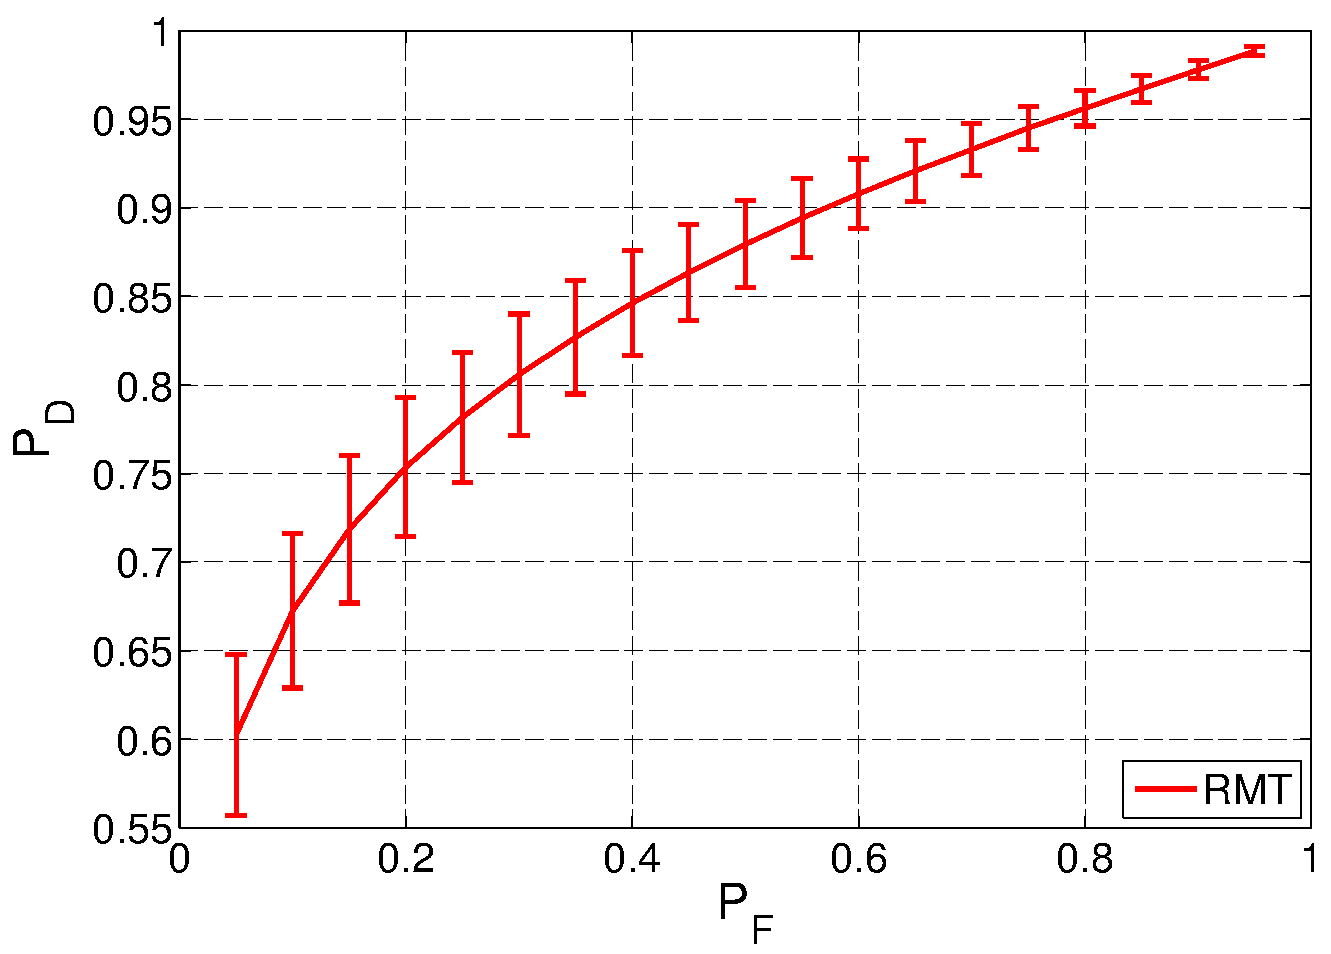
\includegraphics[width=1.5in]{figures/stoch_errorbar_small.pdf}
\label{fig:errorbar_small}
}
\subfigure[$n=200$]{
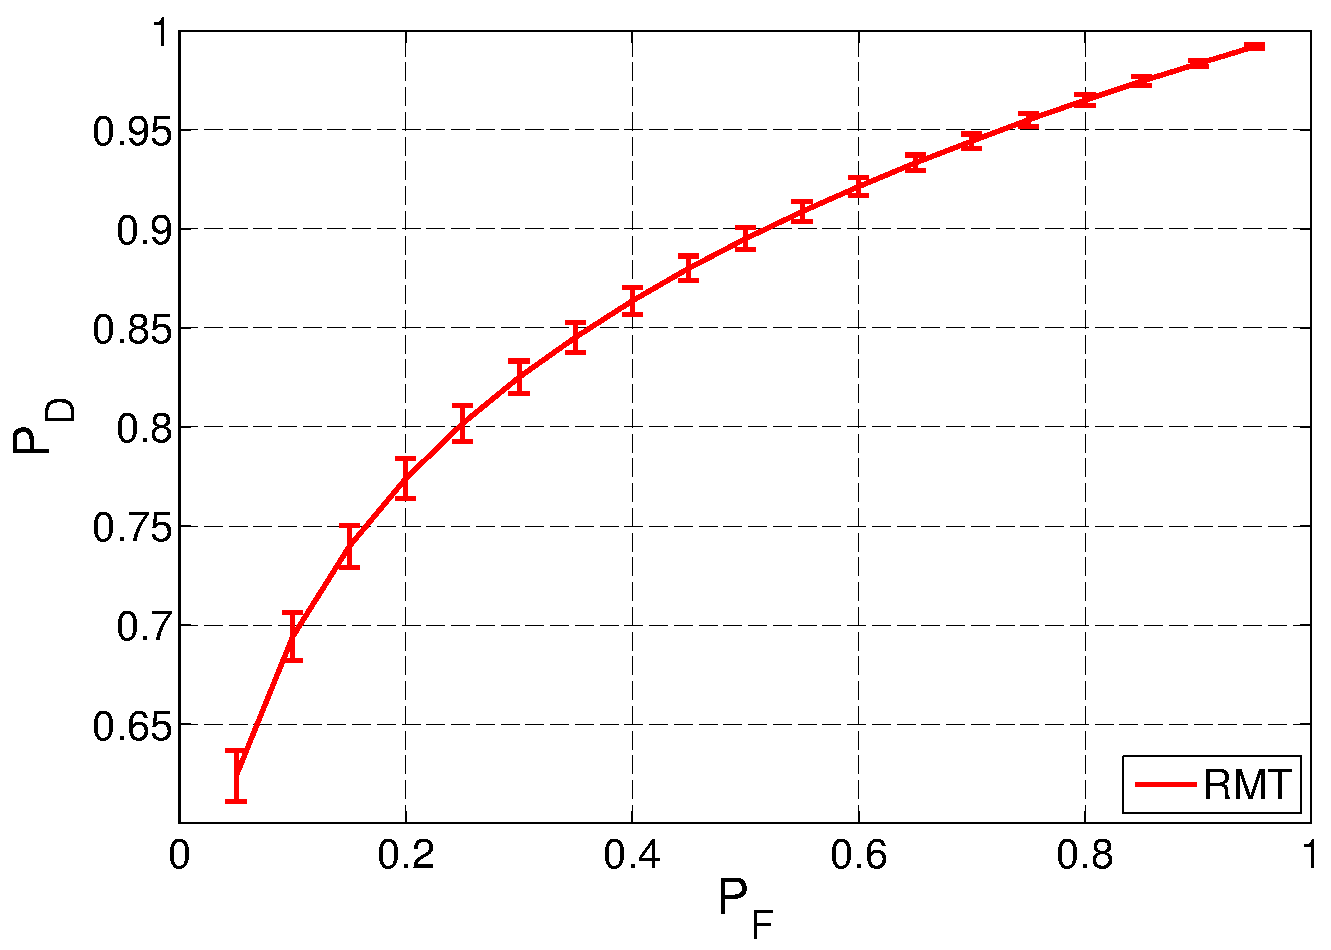
\includegraphics[width=1.5in]{figures/stoch_errorbar_med.pdf}
\label{fig:errorbar_med}
}
\subfigure[$n=1000$]{
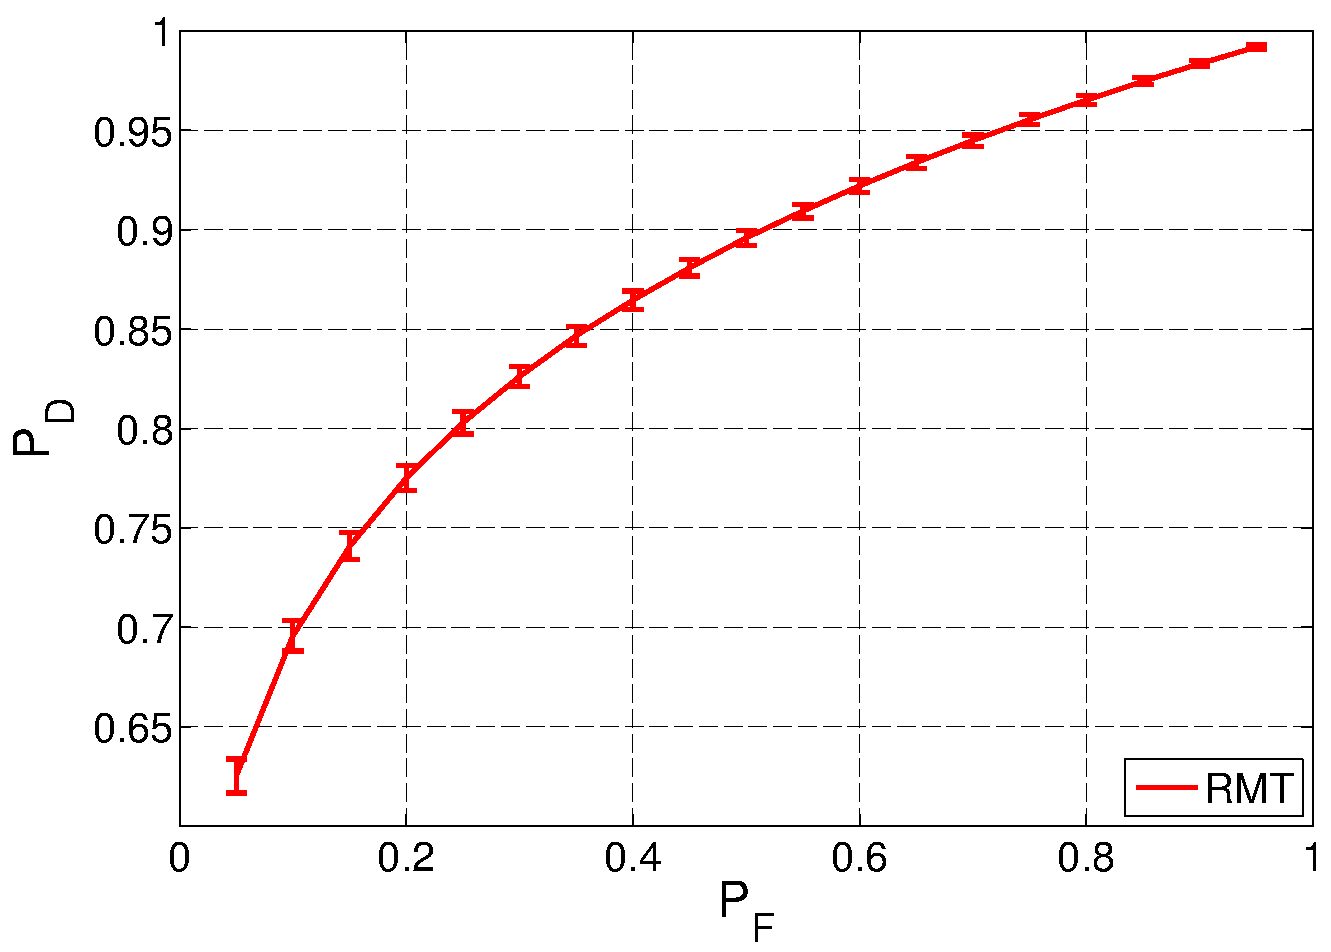
\includegraphics[width=1.5in]{figures/stoch_errorbar_large.pdf}
\label{fig:errorbar_large}
}
\subfigure[Bias]{
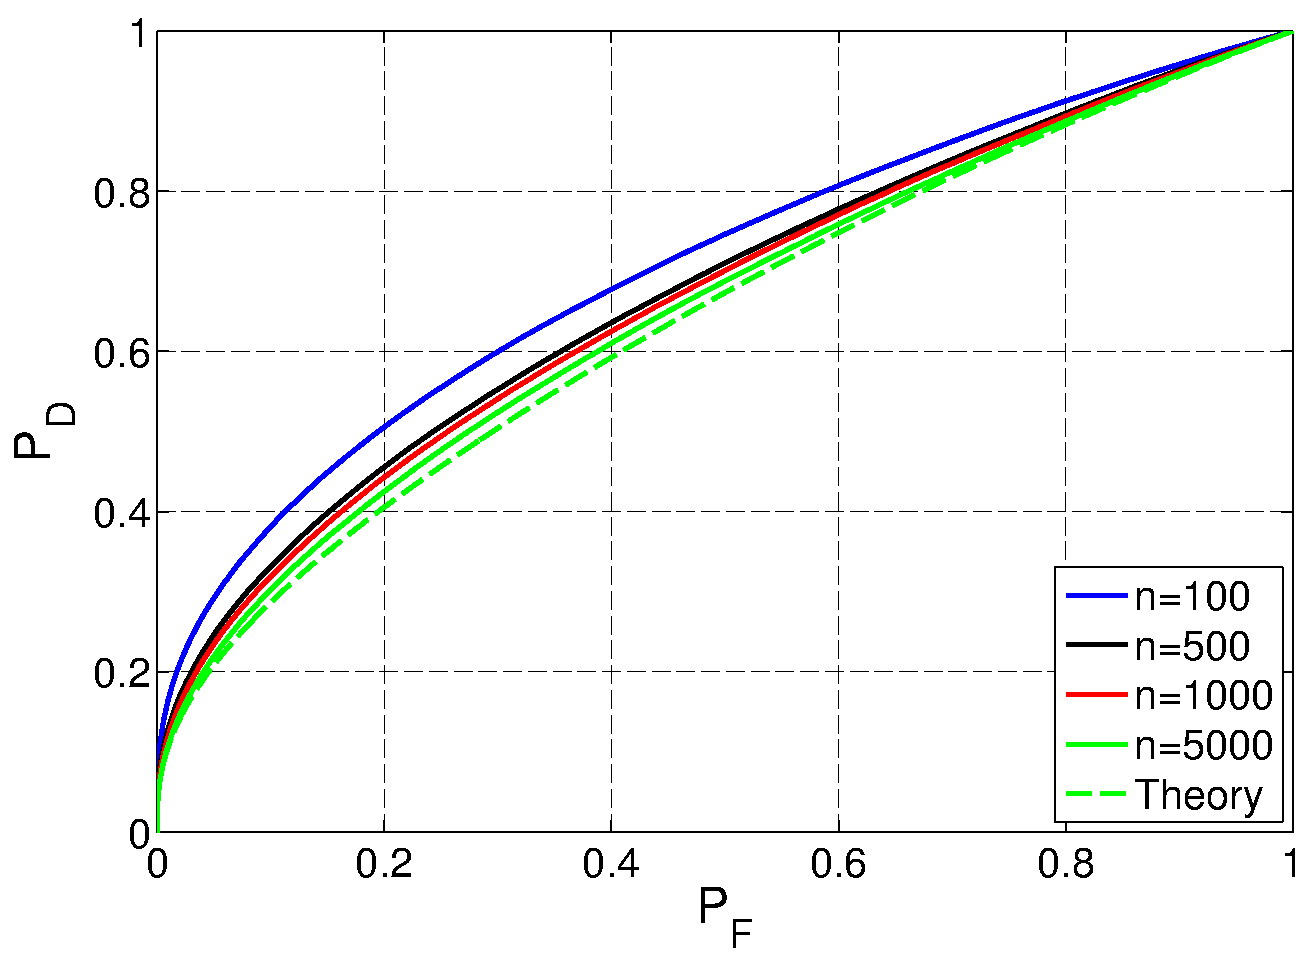
\includegraphics[width=1.5in]{figures/stoch_n_effect.pdf}
\label{fig:stoch_n_effect}
}
\caption{(a)-(c):Empirical ROC curves with one standard deviation errorbars for the stochastic RMT detector. Empirical ROC curves were simulated with $c=2$, $\widehat{k}=k=2$, and $\Sigma =\diag\left(10,5\right)$. The empirical ROC curves were computed using $10000$ test samples and averaged over 100 trials using algorithms 2 and 4 of \cite{fawcett2006introduction}. As both signal variances are above the critical threshold, $k_{\text{eff}} = 2$. For Figure \ref{fig:errorbar_small} $n=50$ and $m=25$. For Figure \ref{fig:errorbar_med} $n=200$ and $m=100$. For Figure \ref{fig:errorbar_large} $n=1000$ and $m=500$. (d): Empirical and theoretical ROC curves for the stochastic plug-in detector. Empirical ROC curves were simulated with $\widehat{k}=k=4$, $n/m=c=20$, $\Sigma=\diag(10, 3, 2.5, 2)$ so that $k_\text{eff}=1$. The empirical ROC curves were computed using $10000$ test samples and averaged over 100 trials using algorithms 2 and 4 of \cite{fawcett2006introduction}. As $n$ increases, the empirical bias in the ROC curves vanishes.}
\end{figure}

The derived detectors and their subsequent theoretical ROC curve predictions rely on the asymptotic approximations which ignore finite $n$ and $m$ correction terms. To examine the validity of the asymptotic approximations and the rate of convergence, we first consider a setting where $\widehat{k}=k=k_\text{eff}=2$ and $c=2$. Figures \ref{fig:errorbar_small}-\ref{fig:errorbar_large} plot the average empirical ROC curve for the stochastic RMT detector as well as one standard deviation error bars for $n=50,200,1000$, respectively. As expected, as $n$ increases the size of the error bars decreases, attesting to the asymptotic convergence of the RMT approximations. Analyzing the rate of convergence (which we conjecture to be $n^{1/2}$) is an important open problem which we shall tackle in future work.

Figure \ref{fig:stoch_n_effect} considers the stochastic plug-in detector under a different setting where $\widehat{k}=k=4$ but $k_\text{eff}=1$ and $c=20$. This value of $c$ corresponds to the sample starved regime where $n > m$. We see that for small values of $n$, the empirical ROC curve is not well approximated by the asymptotic theoretical predictions. However, as $n$ increases, the empirical bias decreases. Theorem \ref{th:other angles} shows that the off diagonal terms in (\ref{eq:cov mat}) asymptotically tend to zero but in the finite $n$ and $m$ case, these terms are $O(1/\sqrt{n})$ and thus not identically zero. For larger rank systems (increased $k$), there are more of these non-identically-zero terms which worsens the approximation quality for fixed, relatively small $n$. As $n$ increases, this bias vanishes.

\subsection{Accuracy of the RMT Approximations}
\begin{figure}
\centering
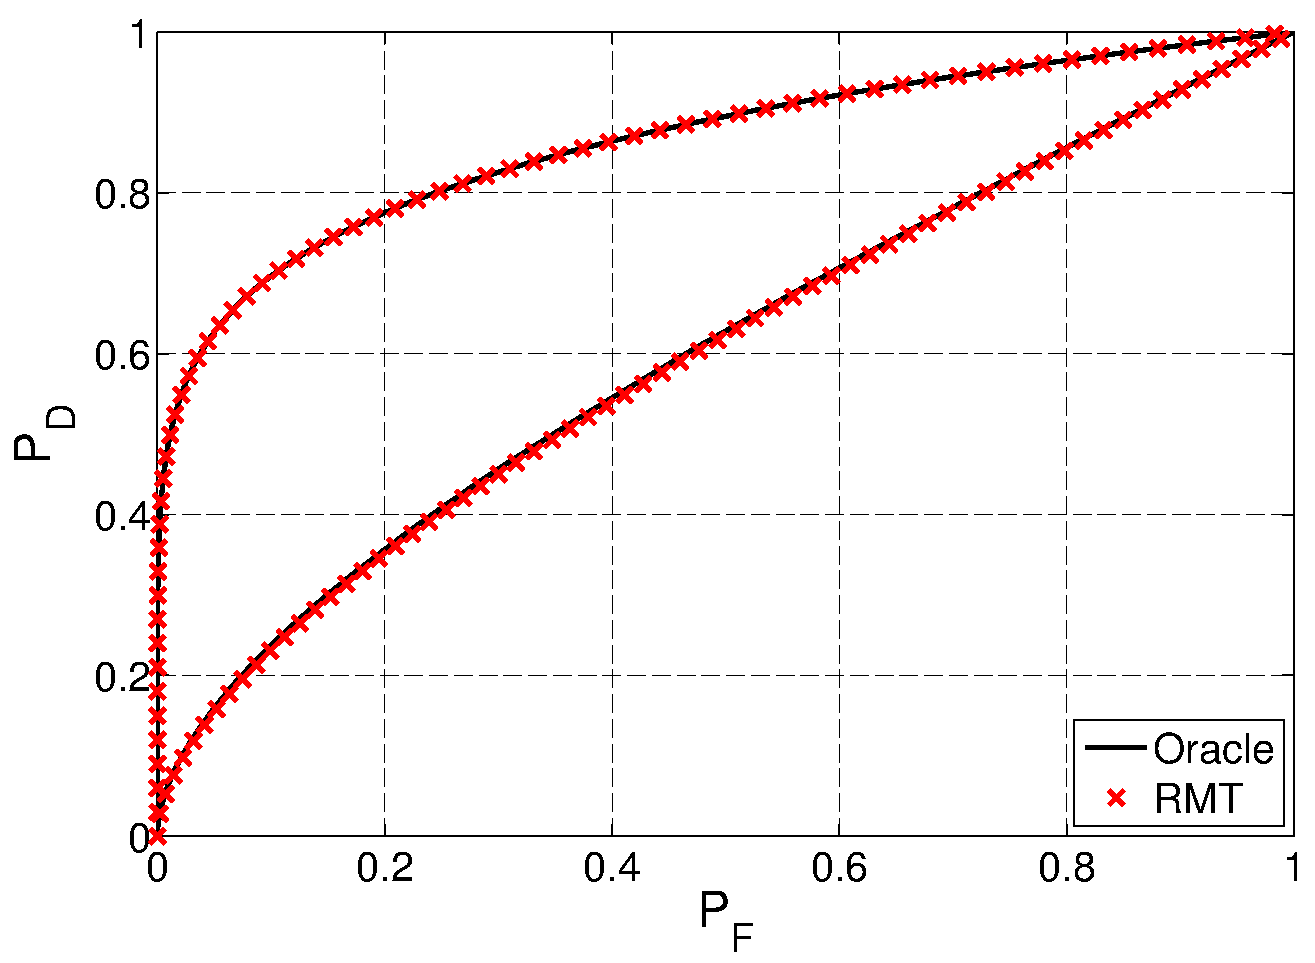
\includegraphics[width=3in]{figures/oracle_rmt.pdf}
\caption{(top curve): Empirical ROC curves for the oracle and RMT stochastic detectors (\ref{eq:oracle_class_stoch}) and (\ref{eq:optimal_class_stoch}) respectively. Empirical ROC curves were simulated with $n=1000$, $m=500$, $\widehat{k}=k=2$, and $\Sigma=\diag(10,5)$. As both $\sigma_1^2=10$ and $\sigma_2^2=5$ are above the critical threshold $\sqrt{c}=\sqrt{2}$, $k_{\text{eff}} = 2$ by equation (\ref{eq:keff}). The empirical ROC curves were computed as descirbed is Section \ref{sec:sim_proto} using $10000$ test samples generated from (\ref{eq:stoch_setup}) and averaged over 100 trials using algorithms 2 and 4 of \cite{fawcett2006introduction}. The stochastic RMT detector realizes the same performance as the oracle detector thereby validating the approximation of Corollary \ref{corr:matrix}. (bottom curve): This is the same setting as the top curve except $\Sigma = \diag(2.5, 1.25)$. In this case, as $\sigma_2^2=1.25< \sqrt{2}$, $k_{\text{eff}} = 1$ by equation (\ref{eq:keff}). Even when $k_\text{eff}$ changes, the stochastic RMT detector is a good approximation to the oracle statistic giving further credibility to Corollary \ref{corr:matrix}.}
\label{fig:oracle_rmt}
\end{figure}

The stochastic RMT detector approximates the oracle detector by employing the RMT approximations, for large $n$ and $m$, developed in Section \ref{sec:rmt}. To test the accuracy of the approximations for finite $n$ and $m$, we examine the empirical performance of both detectors. Figure \ref{fig:oracle_rmt} plots empirical ROC curves for the RMT and oracle stochastic detectors. In the top curves $\widehat{k}=k=k_\text{eff}=2$ and in the bottom curves $\widehat{k}=k=2 > k_\text{eff}=1$. For both values of $k_\text{eff}$, the RMT detector is a good approximation to the oracle detector thereby validating the approximation from Corollary \ref{corr:matrix}.


\subsection{Accuracy of ROC Curve Prediction}

\begin{figure}
\centering
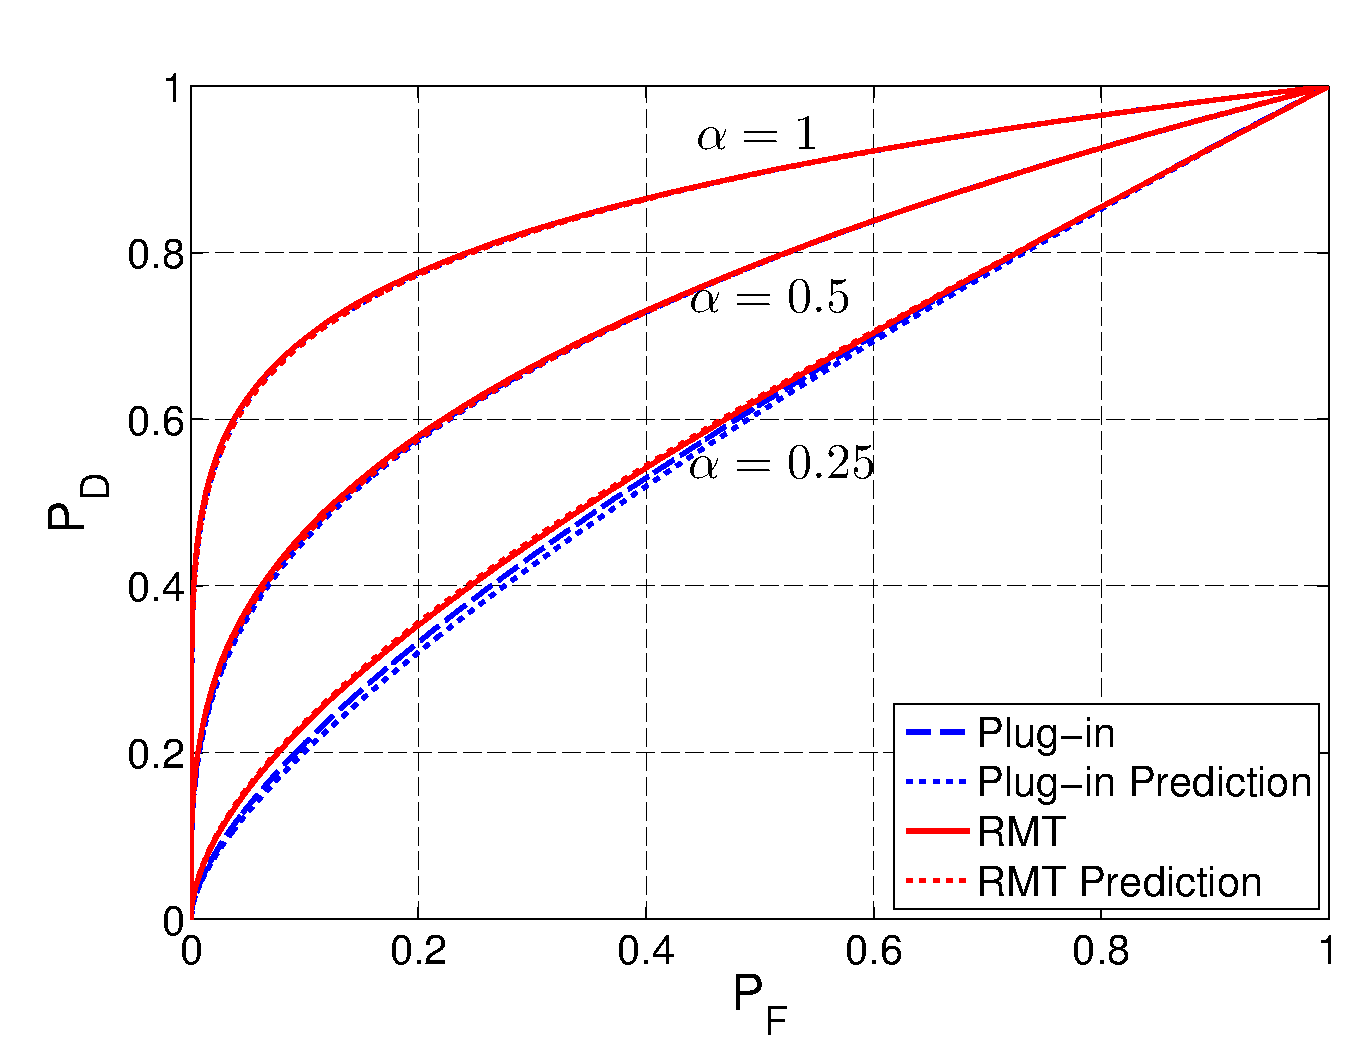
\includegraphics[width=3in]{figures/stoch_roc_pred.pdf}
\caption{Empirical and theoretical ROC curves for the plug-in and RMT stochastic detectors (\ref{eq:plugin_class_stoch}) and (\ref{eq:optimal_class_stoch}) respectively. Empirical ROC curves were simulated as in Figure \ref{fig:oracle_rmt} except with $\Sigma =\alpha\diag\left(10,5\right)$. Results are plotted for $\alpha=1,0.5,0.25$. For $\alpha=1$ and $\alpha=0.5$, $\widehat{k}=k=k_\text{eff}=2$ by (\ref{eq:keff}). For $\alpha=0.25$, $k_\text{eff}=1$. The theoretical ROC curves were computed as described in Section \ref{sec:roc_stoch}. For all values of $\alpha$, all theoretically predicted ROC curves match the empirical results reflecting the accuracy of the approximations employed and the Lugannani-Rice formula. Since $\widehat{k} > k_{\text{eff}}$ when $\alpha=0.25$, we observe a performance gain when using the RMT detector.}
\label{fig:stoch_roc_pred}
\end{figure}

\begin{figure}
\centering
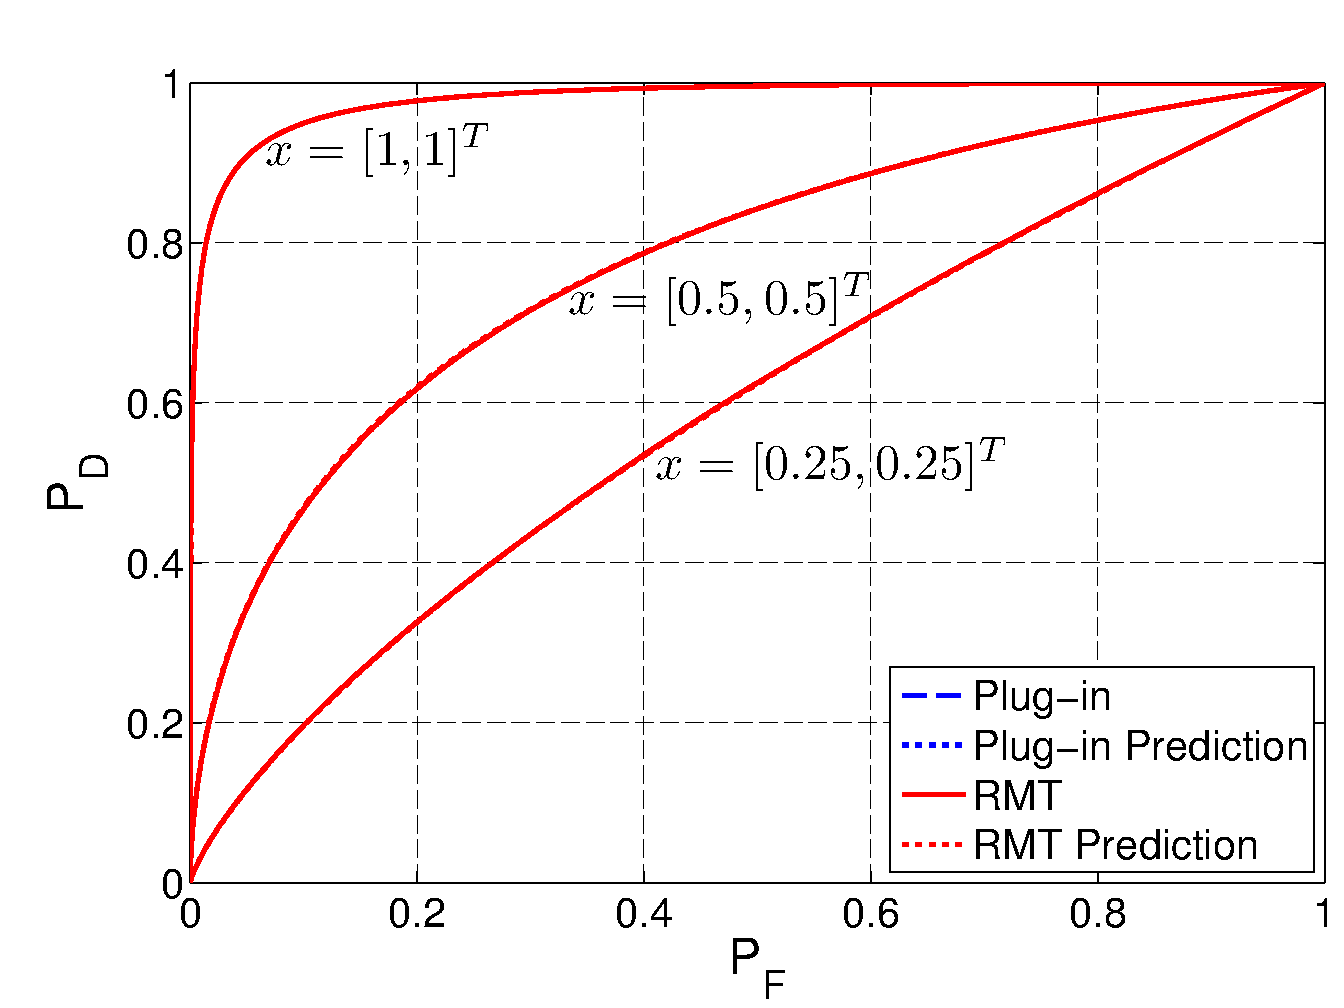
\includegraphics[width=3in]{figures/determ_roc_pred.pdf}
\caption{Empirical and theoretical ROC curves for the plug-in and RMT deterministic detectors (\ref{eq:plugin_class_determ}) and (\ref{eq:optimal_class_determ}) respectively. Empirical ROC curves were simulated as in Figure \ref{fig:oracle_rmt} except with test samples generated from (\ref{eq:determ_setup}) and $\Sigma=\diag(10,5)$ so that $k_{\text{eff}} = 2$. Three values of the deterministic signal vector were used: $x=[1,1]^T$, $x=[0.5,0.5]^T$, and $x=[0.25,0.25]^T$. The theoretical ROC curves were computed using (\ref{eq:roc}). The theoretically predicted ROC curves match the empirical results reflecting the accuracy of Corollary \ref{corr:matrix}. The resulting ROC curves depend on the choice of $x$, however, since $\widehat{k} = k_{\text{eff}}$, the plug-in and RMT detector achieve the same performance for all $x$.}
\label{fig:determ_roc_pred}
\end{figure}

To test the accuracy of the ROC predictions developed in Section \ref{sec:roc_theory} which rely on the random matrix theoretic approximations presented in Section \ref{sec:rmt}, we consider a setting where $\widehat{k}=k = 2$. Figure \ref{fig:stoch_roc_pred} plots empirical and theoretical ROC curves for the plug-in and RMT stochastic detectors for $\Sigma=\alpha\diag(10,5)$ for three choices of $\alpha$. Figure \ref{fig:determ_roc_pred} plots empirical and theoretical ROC curves for the plug-in and RMT deterministic detectors for $\Sigma=\diag(10,5)$ for three choices of the deterministic test vector $x$. The choices of $\Sigma$ and $x$ affect the performance of the resulting detectors.

In both settings, the theoretical ROC curves match the empirical ROC curves thereby validating the accuracy of the random matrix theoretic approximations employed and the accuracy of the saddlepoint approximation to the c.d.f. used in the stochastic derivation. In the stochastic setting, using $\alpha=0.25$ results in $k_\text{eff}=1$. As $\widehat{k}>k_\text{eff}$, the plug-in detector realizes a performance loss. As we might intuitively expect, larger values of $\alpha$ result in better detector performances as larger $\alpha$ yield larger signal variances. In the deterministic setting, larger values of $|x|$ result in better detector performance. However, as the test vector does not affect the value of $k_\text{eff}=\widehat{k}$, the plug-in and RMT detectors achieve the same performance because they have identical statistics.

\subsection{Effect of the Number of Training Samples}

\begin{figure}
\centering
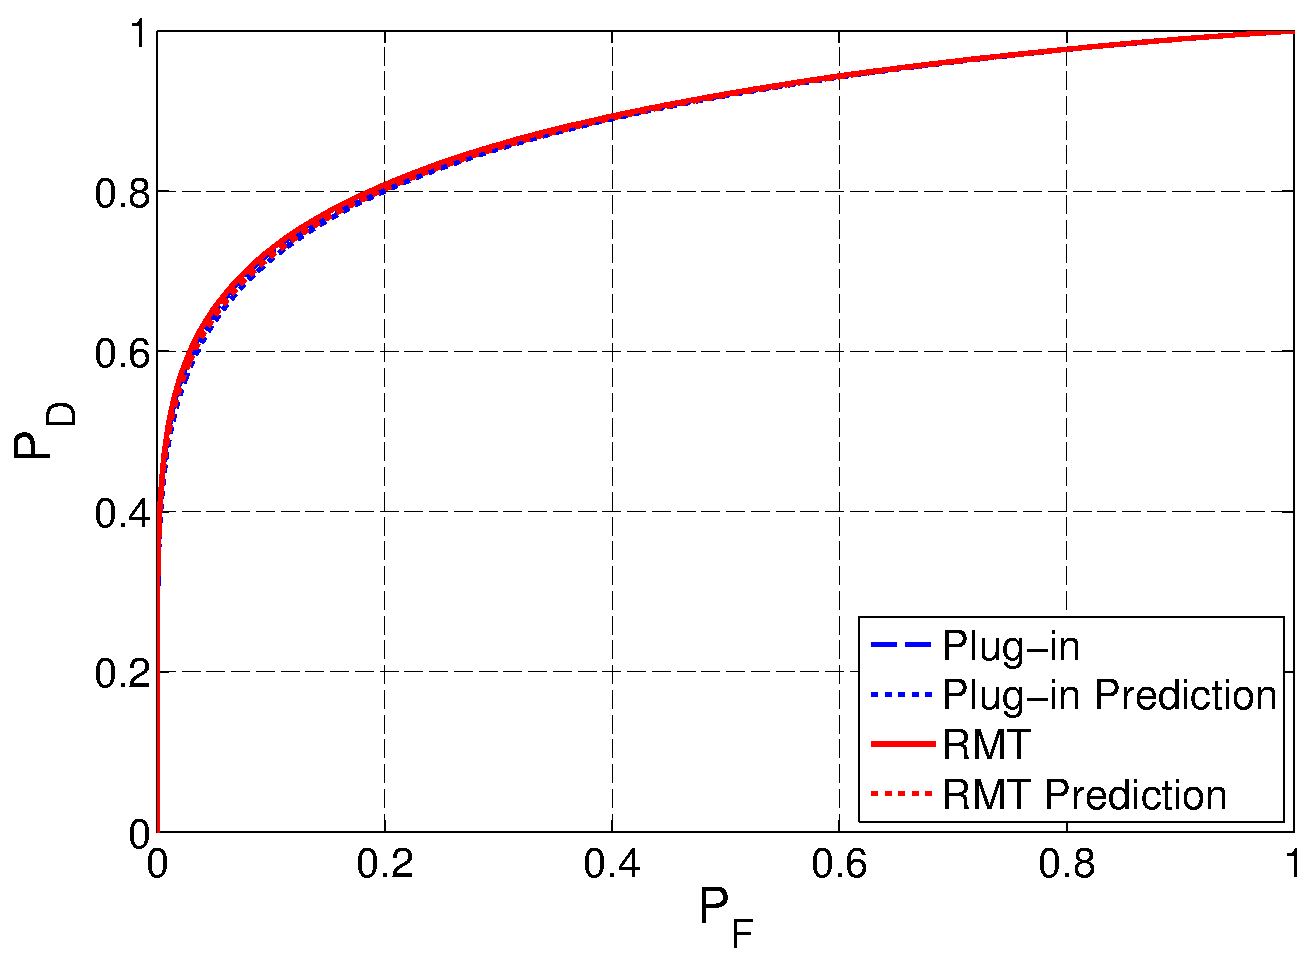
\includegraphics[width=3in]{figures/stoch_m_large.pdf}
\caption{Empirical and theoretical ROC curves for the plug-in and RMT stochastic detectors. This is the same setup as Figure \ref{fig:stoch_roc_pred} except with $n=m=5000$, $\widehat{k}=k=4$ and $\Sigma = \diag({\bf{10,3,2.5,2}})$ so that $k_{\text{eff}}=4$. As the choice of $m$ resulted in $k_\text{eff}=\widehat{k}=4$, the plug-in and RMT detectors achieve relatively the same performance.}
\label{fig:stoch_m_large}
\end{figure}

\begin{figure}
\centering
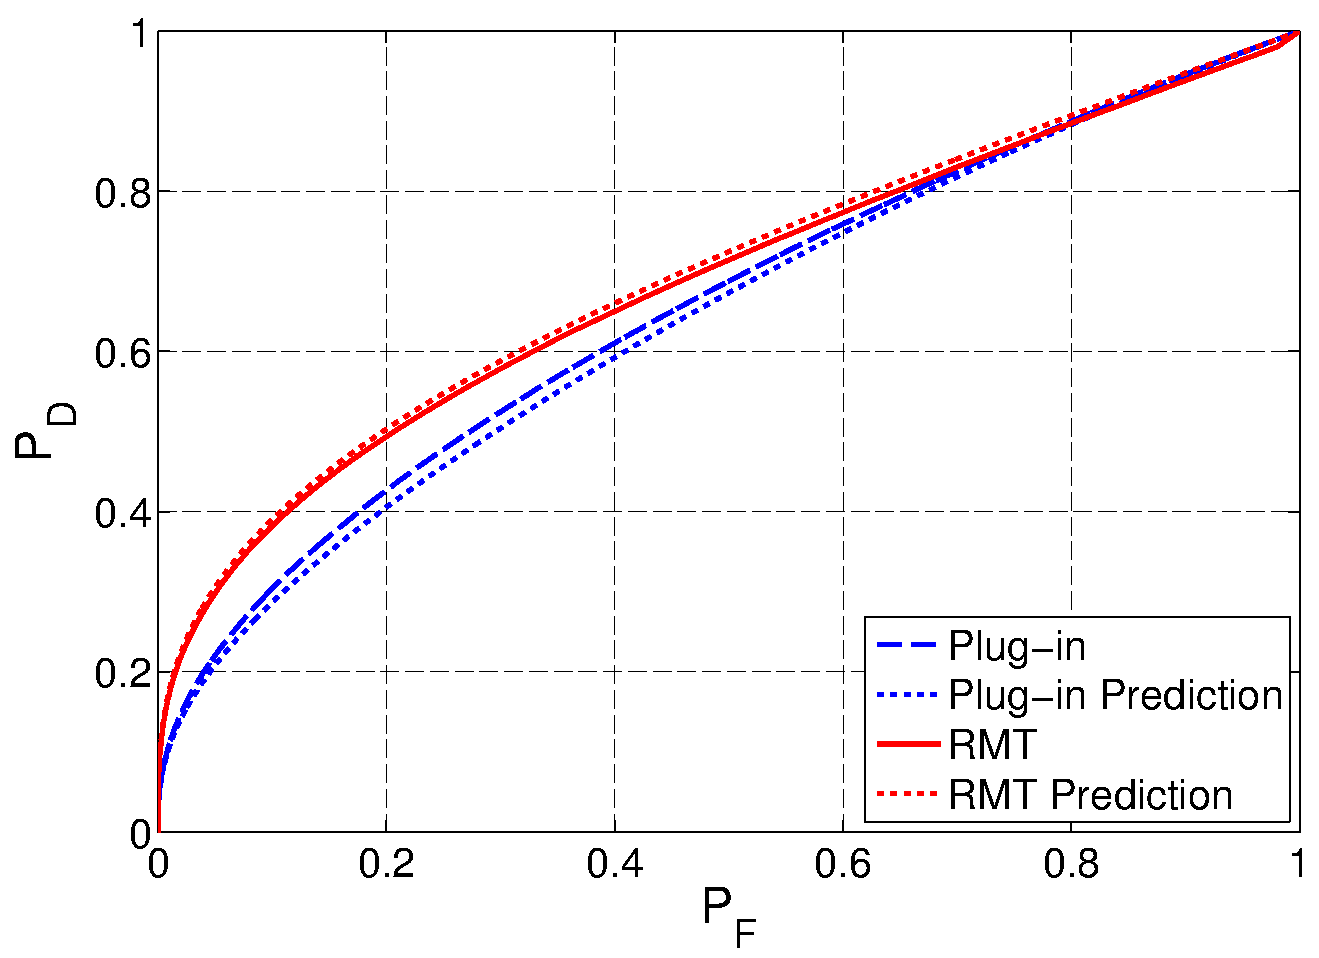
\includegraphics[width=3in]{figures/stoch_m_small.pdf}
\caption{Empirical and theoretical ROC curves for the plug-in and RMT stochastic detectors with the same setup as Figure \ref{fig:stoch_m_large} except with $m=250$ so that $k_{\text{eff}}=1$. As the choice of $m$ resulted in $k_\text{eff}=1<\widehat{k}=4$, the plug-in detector is suboptimal. The disagreement between the theoretical and empirical ROC curves is attributed to finite dimensionality.}
\label{fig:stoch_m_small}
\end{figure}

As derived in Section \ref{sec:rmt}, for a fixed $\Sigma$, the number of training samples, $m$, directly affects $k_\text{eff}$ via (\ref{eq:keff}). To explore how the number of training samples affects detector performance, we consider the stochastic setting where $\widehat{k}=k=4$. Figure \ref{fig:stoch_m_large} investigates the performance when $m=n$ so that $c=1$. With the choice of $\Sigma=\diag(10,3,2.5,2)$, this choice of $m$ results in $k_\text{eff}=\widehat{k}=4$. In this setting, the plug-in and RMT detectors achieve relatively the same performance. Figure \ref{fig:stoch_m_small} chooses $20m=n$ so that $c=20$ and $k_\text{eff}=1$.

In the second setting, the plug-in detector becomes suboptimal because it uses $4=\widehat{k} > k_\text{eff}=1$ subspace components. Whenever $k_\text{eff}<\widehat{k}$ the RMT detector avoids the performance loss realized by the plug-in detector. We could have produced the same effect as this experiment by varying $\Sigma$ instead of $m$ as both of these quantities drive the value of $k_\text{eff}$.

The disagreement between the theoretical and empirical ROC curves is attributed to the finite $n$ and $m$ correction terms which we have neglected. As $k$ increases, there are more off-diagonal terms in the covariance matrix in (\ref{eq:cov mat}) that are not identically zero, as discussed earlier. Theorem \ref{th:other angles} shows that asymptotically these off diagonal terms decay to zero but in the finite $n$ and $m$ case, they are non-zero. In the case of larger $k$, there are more of these non-identically-zero terms thereby worsening the approximation.

\subsection{Effect of $\widehat{k}$}
\begin{figure}
\centering
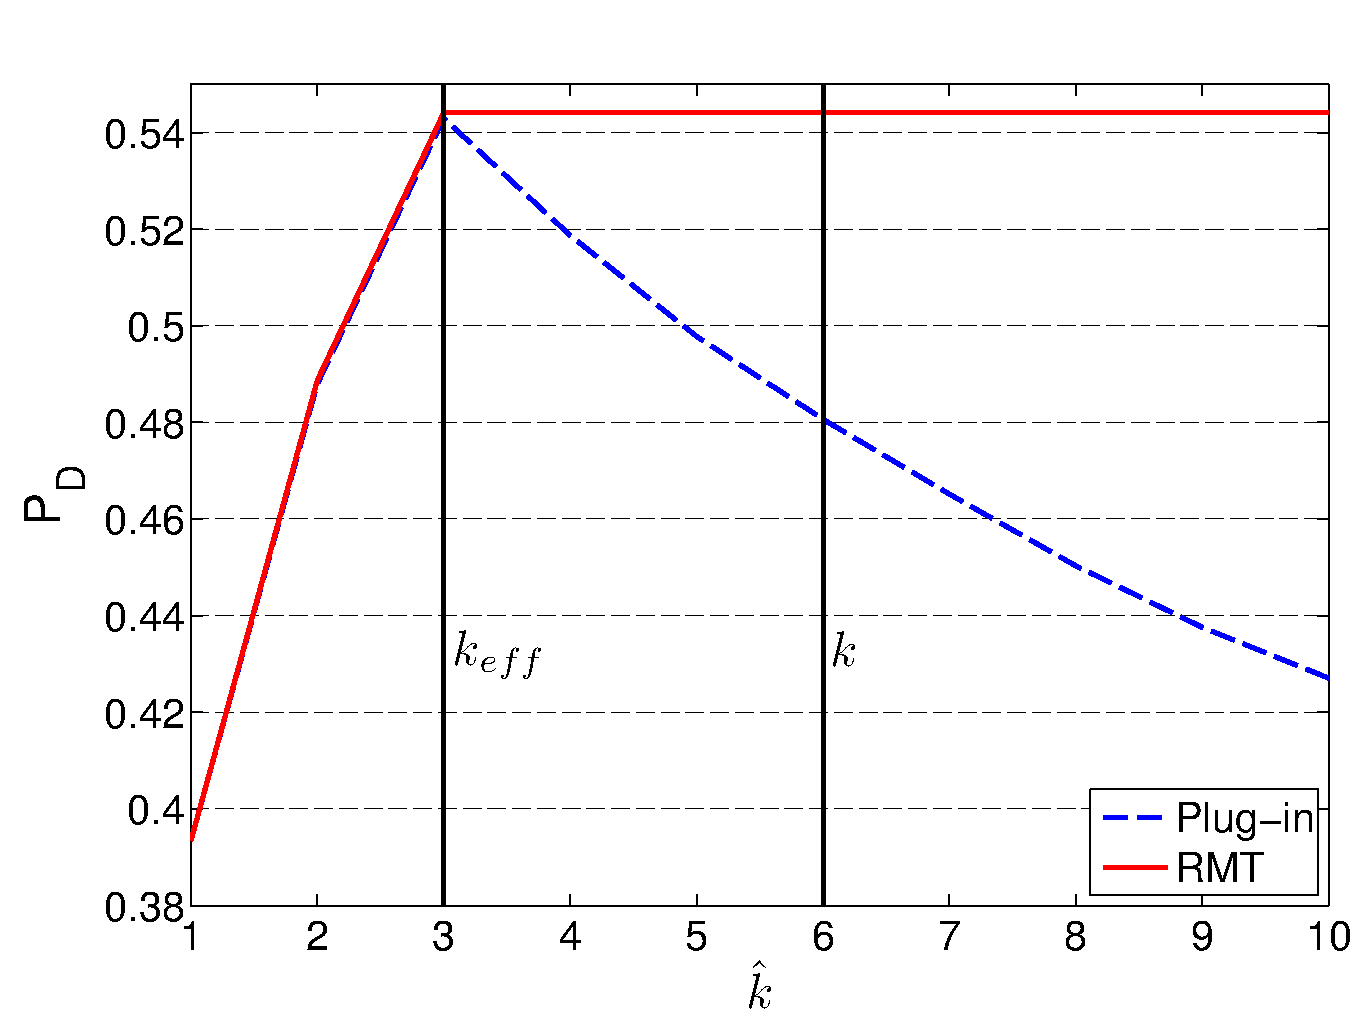
\includegraphics[width=3in]{figures/stoch_khat.pdf}
\caption{Empirical exploration of the achieved probability of detection, $P_D$, for a fixed probability of false alarm, $P_F=0.01$, for various $\widehat{k}$. We are in the same setting as Figure \ref{fig:stoch_roc_pred} except with $k=6$ and $\Sigma = \diag({\bf{10,5,4}},1,0.75,0.5)$ so that $k_{\text{eff}}=3$. The optimal $\widehat{k}$ resulting in the largest $P_D$ is not the true $k$, but rather $k_\text{eff}$.}
\label{fig:stoch_khat}
\end{figure}

Figure \ref{fig:stoch_khat} examines the performance of the plug-in and RMT stochastic detectors as a function of $\widehat{k}$ by plotting the empirically achieved probability of detection for a constant false alarm rate of $0.01$. The result confirms that $k_\text{eff}$ is the optimal choice for $\widehat{k}$. When the plug-in detector uses $\widehat{k} = k_\text{eff}$ it achieves an equivalent performance as the RMT detector.

Setting $\widehat{k} < k_\text{eff}$ drastically degrades performance for both detectors. In this regime, the plug-in and RMT detectors realize the same ROC performance, demonstrating that quantification and exploitation of the subspace estimation accuracy, while useful in ROC performance prediction, does \textit{not} noticeably enhance detection performance. When $\widehat{k} > k_\text{eff}$, the performance of the plug-in detector degrades while that of the RMT detector is stable as if $\widehat{k}=k_\text{eff}$. In other words, we do not pay a price for overestimating the subspace dimension with the RMT detector. This makes sense (and is slightly contrived) because the RMT detector will only sum to a maximum of $k_\text{eff}$ indices as evident in (\ref{eq:optimal_stat_stoch}). In many applications, practitioners might employ the ``play-it-safe'' approach and set $\widehat{k}$ to be significantly greater than $k_\text{eff}$. The performance loss caused by adding each uninformative subspace, as seen in Figure \ref{fig:stoch_khat}, constitutes evidence to the assertion that overestimating the signal subspace dimension is a bad idea. When $k_\text{eff} < k$, even perfectly estimating the subspace dimension (i.e. setting $\widehat{k} = k$) is suboptimal.


\subsection{Effect of Averaging Multiple Test Samples}
\begin{figure}
\centering
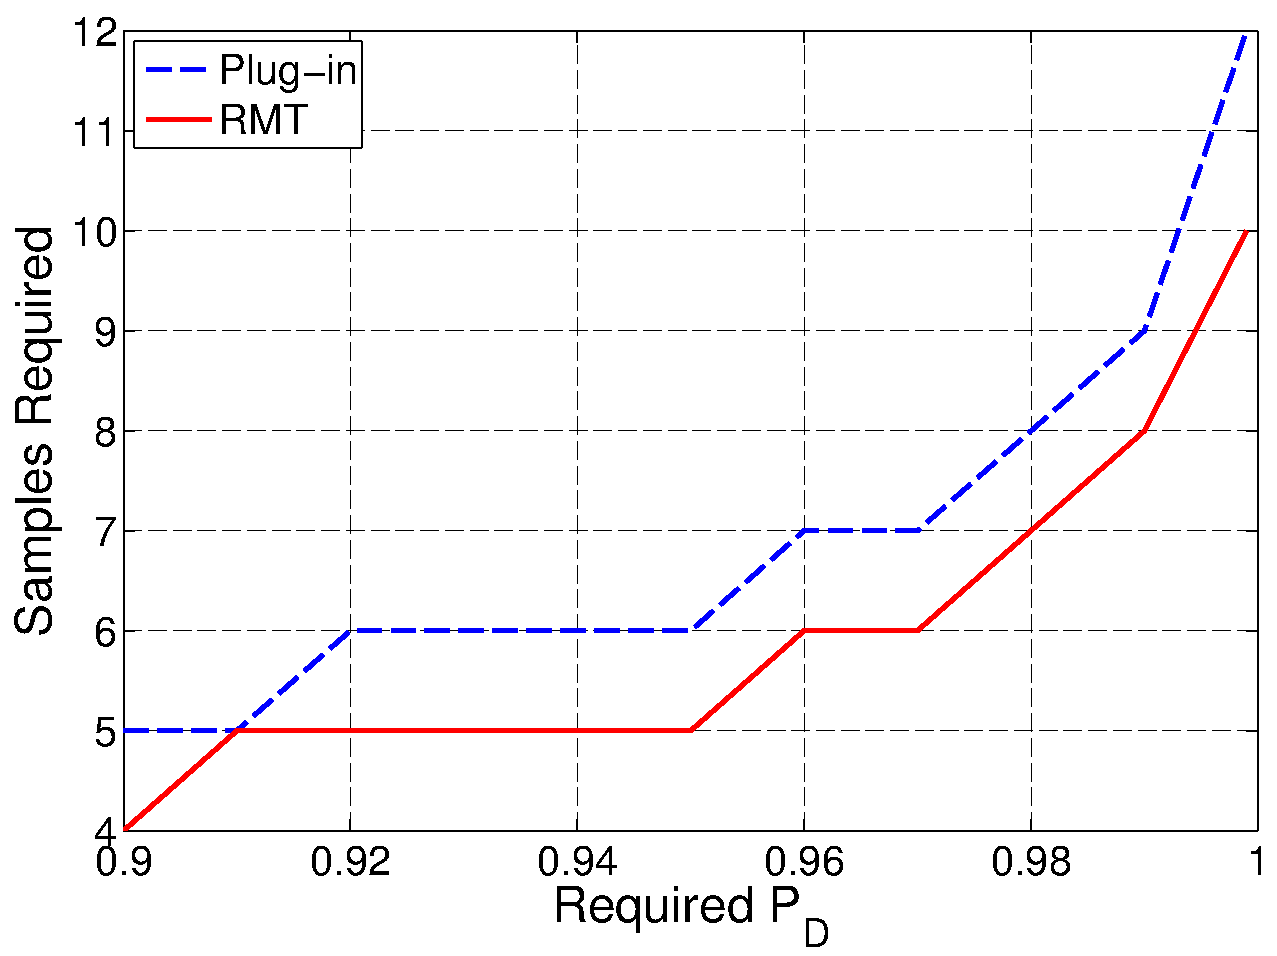
\includegraphics[width=3in]{figures/stoch_samples.pdf}
\caption{Empirical exploration of the number of test samples required to achieve a desired $P_F=0.001$ for different $P_D$. In this setup, the test statistic for each detector is averaged over multiple independent test samples. We are in the same setting as Figure \ref{fig:stoch_khat} except with $\widehat{k}=k=6$. Because the RMT detector only uses informative subspace components, it can average less test samples than the plug-in detector to achieve a desired $(P_F, P_D)$ pair.}
\label{fig:stoch_samples}
\end{figure}

Figure \ref{fig:stoch_samples} considers the performance of the plug-in and RMT stochastic detectors when averaging multiple independent test samples to form the test statistic. In this setting, $k_\text{eff} =3$ and the plug-in detector sets $\widehat{k} = k = 6$. The RMT detector can average less samples than the plug-in detector to achieve a desired $(P_F, P_D)$ pair. Since the RMT detector discards the uninformative signal subspace components, each test sample is pruned to ignore noisy components. As the plug-in detector includes uninformative subspace components, its test statistic is noisier and so it must be averaged over more samples to achieve a desired level of detection accuracy. This requires waiting for additional test vectors thereby increasing the time-to-decision.

\subsection{Effect of $x$ in the Deterministic Setting}
\begin{figure}[t]
\centering
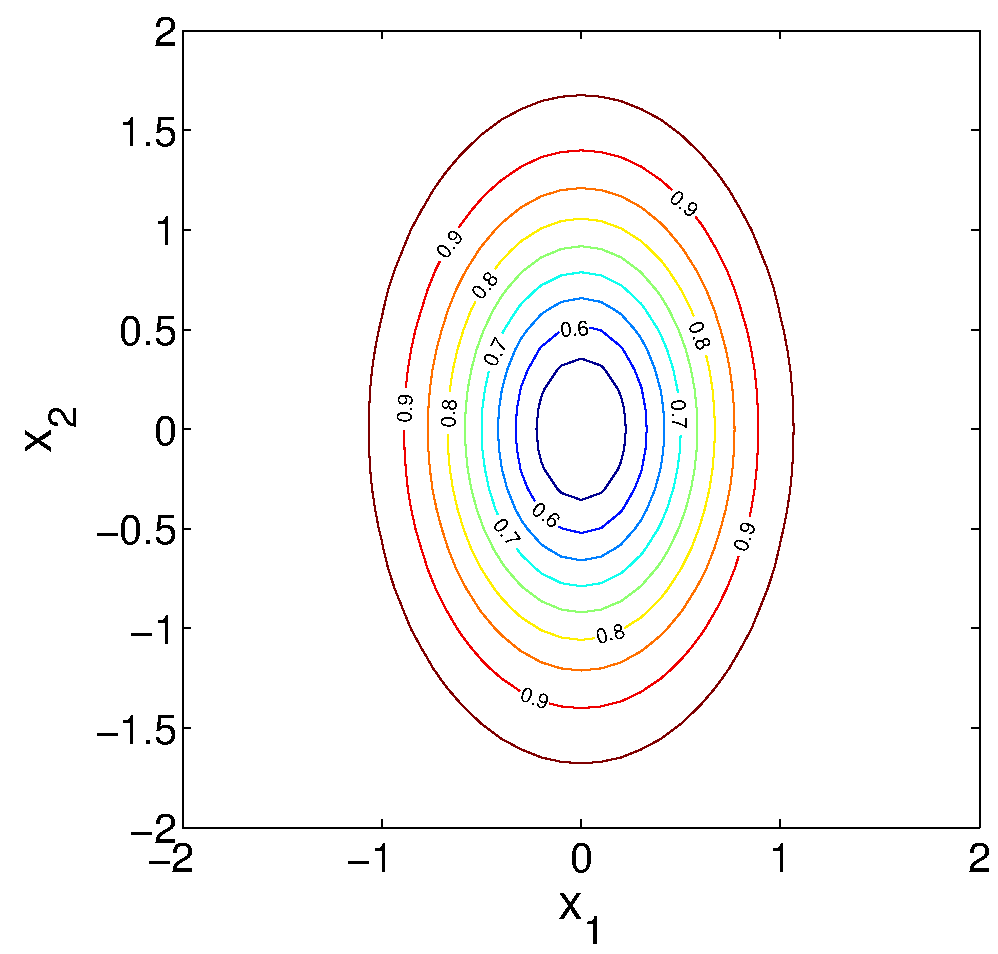
\includegraphics[width=2.5in]{figures/determ_rmt_theory_contour_large_keff.pdf}
\caption{Contour plot of the theoretical area under the ROC curve (AUC) for the deterministic RMT detector. We are in the same setting as Figure \ref{fig:determ_roc_pred}. As both signal variances are above the critical threshold, $k_{\text{eff}} = 2$. We see that the orientation of the contours follows the inverse signal variance structure. As $\sigma_1^2=10 > \sigma_2^2=5$, the vertical contour axis is longer than the horizontal one. }
\label{fig:determ_rmt_theory_contour}
\end{figure}

\begin{figure}[t]
\centering
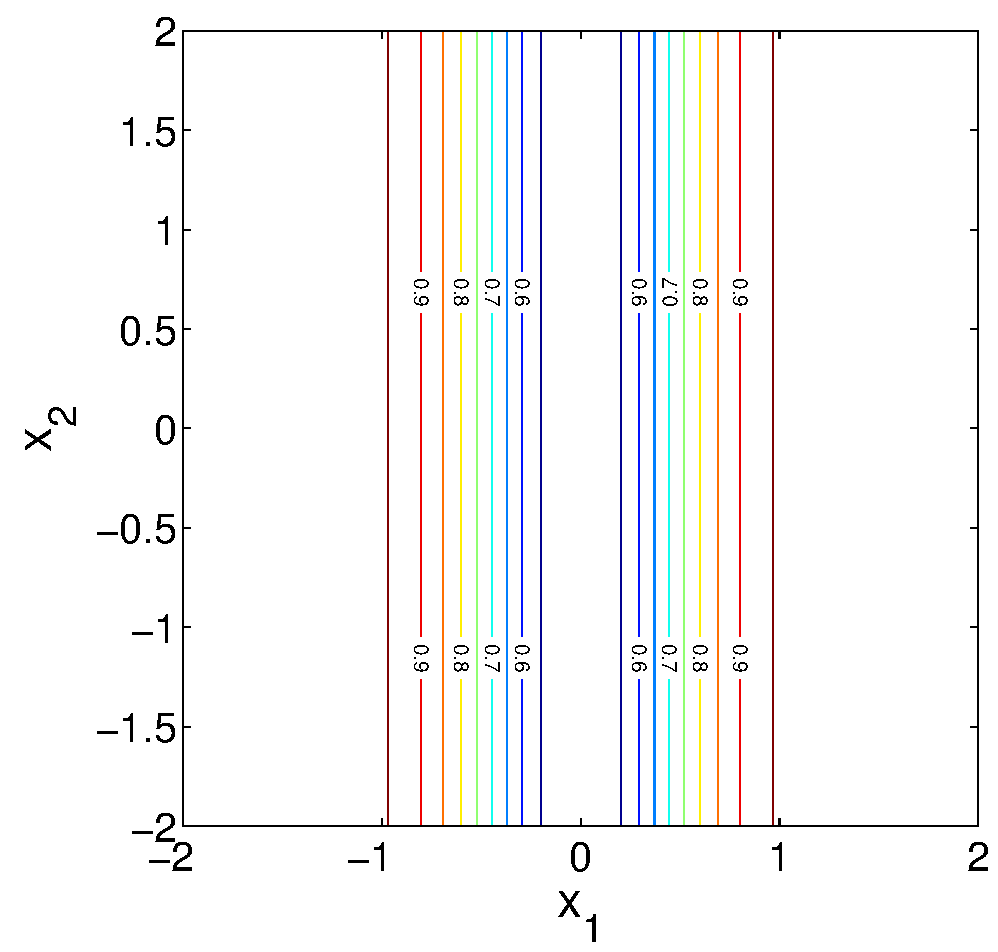
\includegraphics[width=2.5in]{figures/determ_rmt_theory_contour_small_keff.pdf}
\caption{Contour plot of the theoretical area under the ROC curve (AUC) for the deterministic RMT detector. We are in the same setting as Figure \ref{fig:determ_rmt_theory_contour} except that $\Sigma=\diag(10,1)$. As only the first signal variance is above the critical threshold, $k_{\text{eff}} = 1$. Because of this, the deterministic RMT detector will ignore the second, uninformative component of the test vector. We see this manifested in the contour plot as all contours are vertical lines indicating that $x_2$ has no impact on the RMT detector.}
\label{fig:determ_plugin_theory_contour}
\end{figure}

As seen in the derivation of the theoretical deterministic ROC curves, the choice of the signal vector, $x$, affects the performance of the detector through the non-centrality parameter, (\ref{eq:delta}), of the noncentral chi-square distribution. To explore the effect that $x$ has on detector performance, we consider the setting where $\widehat{k}=k=2$. Figures \ref{fig:determ_rmt_theory_contour} and \ref{fig:determ_plugin_theory_contour} plot the area under the ROC curve (AUC) for various choices of $x$ for the theoretical RMT detector for two choices of $\Sigma$.

As seen in Figure \ref{fig:determ_rmt_theory_contour}, because $\widehat{k}=k_\text{eff}$, larger $|x|$ increase the AUC. Intuitively this makes sense because larger $|x|$ increase the non-centrality parameter, which further separates the conditional distributions of the test statistic under each hypothesis, resulting in better detection ability (higher AUC). The AUC contour lines have major axes inversely proportional to the training data signal covariance matrix, $\Sigma$. In this example, $\sigma_1^2 > \sigma_2^2$; increasing $|x_1|$ increases the AUC more than increasing $|x_2|$. In other words, as $\sigma_1^2 >\sigma_2^2$, to achieve the same increase in AUC, we would need to increase $|x_2|$ more than $|x_1|$. This is evident in the geometry of the contours.

However, in Figure \ref{fig:determ_plugin_theory_contour} the choice of $\Sigma$ results in $k_\text{eff}=1<\widehat{k}=2$. We see the geometry of the AUC contour lines change to vertical lines. This makes sense because the second subspace component is uninformative. Therefore, changes in $|x_2|$ do not affect the performance of the detector, resulting in vertical AUC contour lines.

By placing a standard normal prior on $x$, the stochastic detector may be viewed as the expectation over all deterministic detectors. In fact, we can place any prior on $x$ and obtain a different stochastic detector by taking the expectation over all deterministic detectors with a given prior. This facilitates ROC performance curve analysis over non-Gaussian priors on $x$. 